\documentclass[../rapport.tex]{subfiles}
\graphicspath{{\subfix{ressources/photos_diagrammes/app2/}}}

\begin{document}

Le diagramme de cas d'utilisation à été assez simple à réaliser car il a suffit de se baser sur l'application 1 et de bien comprendre les consignes.
Il constitue la structure de l'application pour les institutions. \\
Le diagramme de cas d'utilisation 2 partage plusieurs points communs avec le diagramme de cas d'utilisation 1 ce qui facilitera l'implémentation par la suite. De plus, il est moins complexe et moins lourd que ce dernier.

\begin{figure}[h!]
	\centering 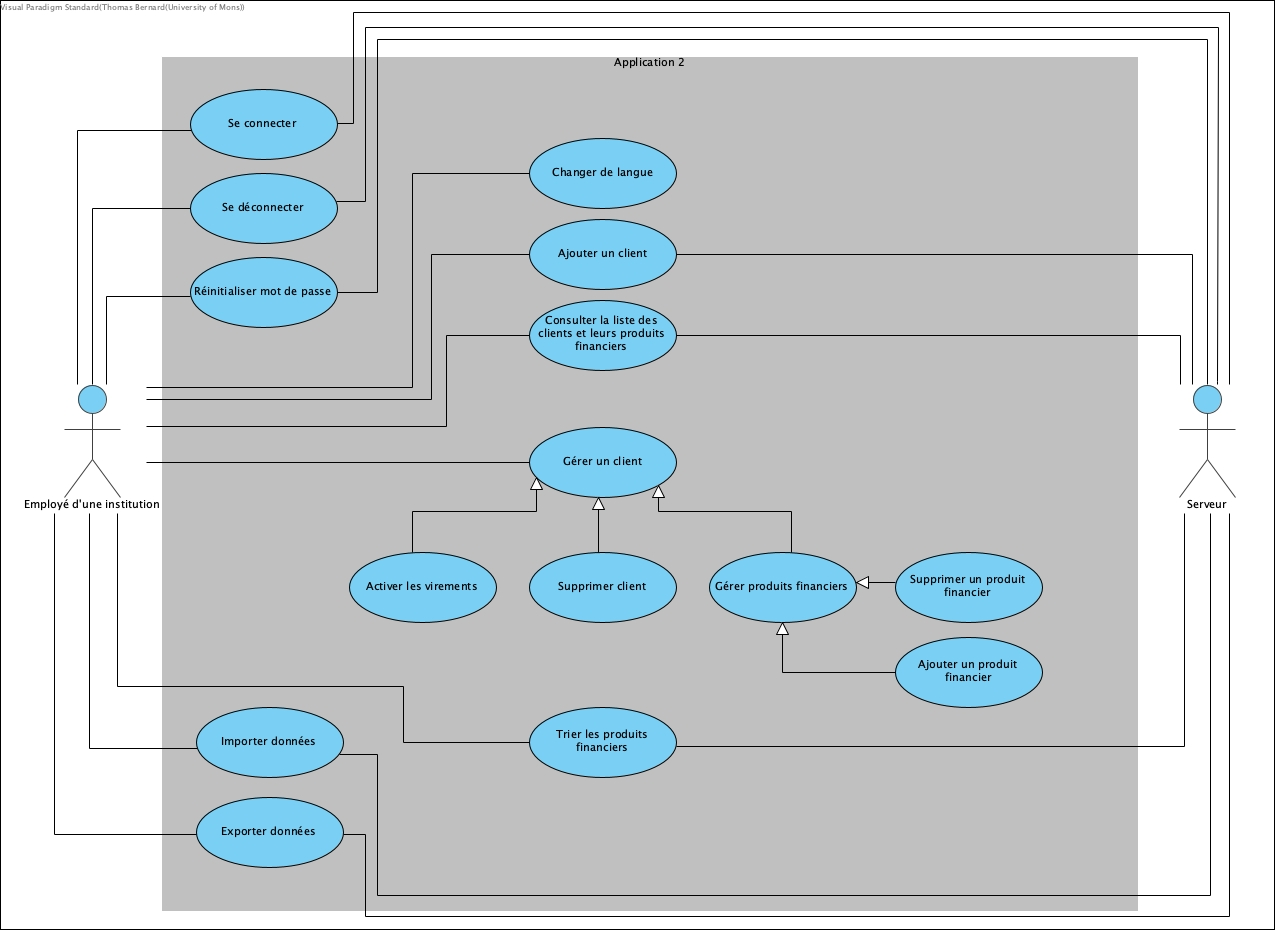
\includegraphics[scale=0.30]{ressources/photos_diagrammes/app2/use_case_app2.jpg}
\end{figure}

\end{document}
